% TEX compiler = luatex
% copyright arturo salinas-aguayo 2025
\documentclass[12pt]{article}

\usepackage{graphicx}
\usepackage{amsmath}
\usepackage{array}
\usepackage{amsfonts}
\usepackage{fancyhdr}
\usepackage{geometry}
\usepackage{circuitikz}
\usepackage{subfigure}
\usepackage{caption}
\usepackage{karnaugh-map}
\usepackage{bm}
\usepackage{float}

\geometry{letterpaper, margin=1in}
\graphicspath{ {../../images/} }

% Header and Footer
\pagestyle{fancy}
\fancyhf{}
\fancyhead[L]{ECE 2001 - Lab 02: The Node Voltage Method}
\fancyhead[R]{\thepage}
\setlength{\headheight}{15pt}

\author{Arturo Salinas-Aguayo}
\title{Lab 02: The Node Voltage Method}
% theorem set
\newtheorem{example}{Example}
% Example block environment
\newenvironment{examp}
{\vspace{0.5cm}
 \hrule
\vspace{0.5cm}
\begin{example}}
{\hrule
\vspace{0.5cm}
\end{example}}

\begin{document}
\newcommand{\closure}[2][3]{%
	{}\mkern#1mu\overline{\mkern-#1mu#2}}
\newcommand\ncoverline[1]{\mkern1mu\overline{\mkern-1mu#1\mkern-1mu}\mkern1mu}
% Title Page
\begin{titlepage}
	\centering
	\vspace*{3cm}
	\huge\textbf{Lab 02: The Node Voltage Method}\\
	\vspace{5cm}
	\Large\textbf{Arturo Salinas-Aguayo}\\
	\normalsize
	ECE 2001 Electrical Circuits\\
	Dr. David J. Giblin, Section 331.660.701.810-1253\\
	Mechanical Engineering Department
	\vfill
	
\includegraphics[scale=0.1]{uconnlogo}\\
	College of Engineering, University of Connecticut\\
	\scriptsize{Coded in \LaTeX}
	\vspace*{1cm}
\end{titlepage}
\tableofcontents
\newpage
\section{Abstract}
The node voltage method is the backbone of dc electrical circuit analysis. It
offers a precise way to map out a circuit and create references to each node
with regard to another. The course starts out detailing the Branch Current
method, which will always work, however once complicated circuits are
introduced, this method begins to show its limitations. Additionally, many times
the inner workings of a circuit are of no importance and the relationship
between the voltage at the output terminals compared to the input terminals is
all that is desired. With branch current, the entire circuit must be ``solved"
which is simply not practical or feasable from a cost perspective. Time is money
and an engineer can prove their worth by making quick and accurate calculations
which do not necessarily include all the tiny branch currents and voltage drops
where not important.
\newpage
\section{Introduction}
The \textit{Node Voltage Method} is a way to formulate the different nodes in
which three or more different components are connected to and reference them to
each other or a common reference point, commonly denoted as a digital ground.

This experiment starts off with some napkin math on the calculation of a few
simple circuits which demonstrate the versatility of the method. The
practicality of the application is then enforced by building the circuits in
hardware utilizing the Protoboard and resistors included in the experiment kit.

The experimental work concludes with calculations within the PSpice simulation
suite. This is not the first time that this is used in the course, however as
more components are introduced, more features and capabilities of the software
suite are shown.
\section{Theory}
\subsection{The Node Voltage Method}
As stated in the abstract of this document, a node voltage is the potential
difference between any given node and some other node that has been denoted as
the \textit{reference node}. The reference node is usually denoted as the
\textit{ground}.

Current always flows from the node with the higher potential to the node with
the lower potential. Utilzing the passive sign convention and knowledge gained
from previous experimental work, components can be assigned polarities which
correspond to the purpose that they serve within the circuit.

For example, a DC voltage source which is supplying power to a circuit has
current pointing in towards the positive terminal, while a DC voltage source
that is absorbing power will have the current flowing the other direction. The
overall direction of the current flow, as stated earlier, has to do with the
magnitude of the potential of the nodes surrounding the component.

Taking a step back, one may realize that this will change depending on what
ground the circuit analyzer chooses and rush to point out that this will lead to
problems in the analysis. In actuality, and only once one convinces themselves
by repeated experimentation, the specific location of the reference node does in
fact not matter in the grand scheme of the analysis as long as the rules are sound
and the laws are obeyed, with a consistent use of \textit{discipline} in the
passive sign convention, the results will turn out equal.

\subsubsection{Kirchoff's Current Law}
The \textit{Node Voltage Method} relys on heavy use of Kirchoff's Current Law
which was heavily explained in Lab 01's lab report, hence I will cover it
briefly here.
\[
	\sum i_{total} = i_1 + ... + i_p = 0\]
Each node gets its own equation set to 0, set in reference to all other nodes in
the circuit. This results in an amount of equations that is equal to the number
of essential nodes minus one, the reference node.

Recall that current, $i$, is equivalent to
$\frac{\upsilon}{R}$ and a large portion of learning comes from the realization
that when utilizing the node voltage method, one solves for missing voltages,
although the KCL equation is a sum of currents. Confusing at first, but with
with some repeated reps, this becomes painfully simple, which is good.

\subsubsection{Special Cases}
There are additional cases in which this may become even more simple, for
example with a dedicated voltage source in series with nothing else within a
branch, the node voltage value is simply the value of the source itself.
Additionally, if there is a voltage source inbetween two nodes, the nodes may be
combined to form a single node, as long as the missing current is handled
accordingly.

\subsubsection{The Big Picutre}
Eventually, one finds the voltages utilizing linear algebra and the circuit can
be solved for a modicum of values, or as seen later on in analysis, simplified
to an equivalent simpler circuit. The node voltage method relies heavily on
established laws, so it always holds true. While sometimes cumbersome, if the
analyzer finds themselves in a troubled predicament with another method, falling
back to this is always an option.

\section{Experiemntial Procedures}
\subsection{Circuit One}
This portion requires finding the expected node voltage, $V_1$, with the
assumption that the bottom node is the reference node for the circuit. Refer to
Figure \ref{fig:circuit1}.
\begin{figure}[H]
	\centering
	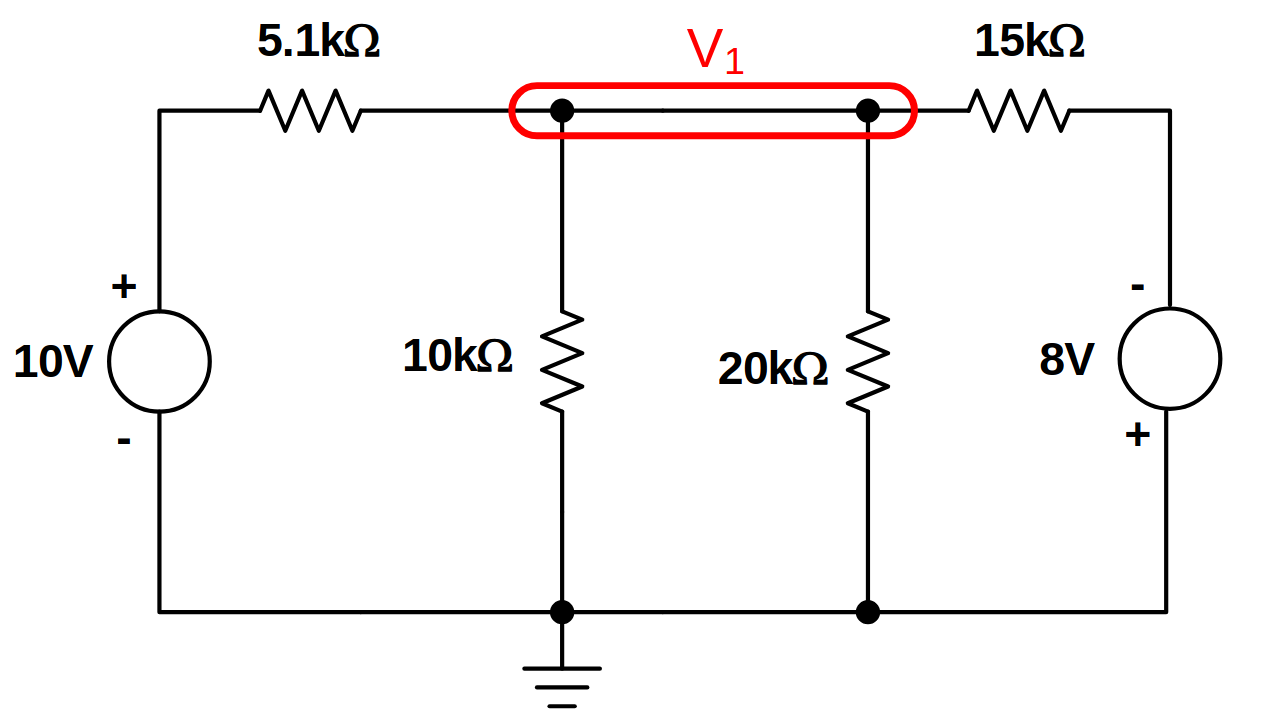
\includegraphics[width=1\textwidth]{06_01}
	\caption{A Simple DC Resistive Circuit}
	\label{fig:circuit1}
\end{figure}
Analytically, there are two essential nodes. Hence, we have one equation and one
unknown, $V_1$.
The equations are setup in units of $k\Omega$, $V$, $mA$, and $mW$ to save
complexity and obfuscation of the math.
\[
	\frac{V_1 - 10}{5.1} + \frac{V_1}{10} + \frac{V_1}{20} + \frac{V_1 + 8}{15} =
	0
\]
\[	V_1 = 3.458 V\]

The results and discussion portion elaborates on the experimental findings of
building this circuit.
\subsection{Circuit Two}
This portion requires solving for multiple unknowns. Referring to Figure
\ref{fig:circuit2}, there are four unknown essential branch voltages, and
therefore will require 3 KCL equations to find 3 unknown voltages. $V_x = 5V$.

The equations are setup in units of $k\Omega$, $V$, $mA$, and $mW$ to save
complexity and obfuscation of the math.
\begin{figure}[H]
	\centering
	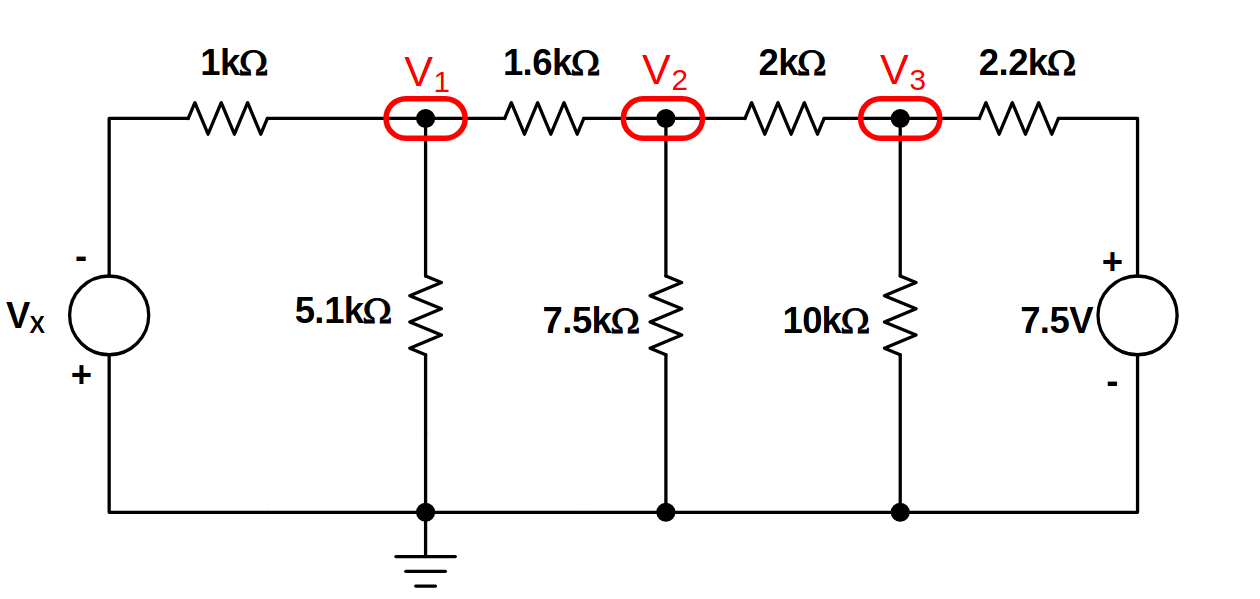
\includegraphics[width=1\textwidth]{06_02}
	\caption{A Slightly More Complex DC Resistive Circuit}
	\label{fig:circuit2}
\end{figure}
\[
	\frac{V_1 + 5}{1} + \frac{V_1}{5.1} + \frac{V_1 - V_2}{1.6} = 0
\]
\[
	\frac{V_2 - V_1}{1.6} + \frac{V_2}{7.5} + \frac{V_2 - V_3}{2} = 0
\]
\[
	\frac{V_3 - V_2}{2} + \frac{V_3}{10} + \frac{V_3 - 7.5}{2.2} = 0
\]
Rearranging and putting each equation into general form:
\begin{align*}
	14.86V_1 - 5.1V_2 + 0V_3 & = -40.8 \\
	-15V_1 + 30.2V_2 - 12V_3 & = 0     \\
	0V_1 - 11V_2 +23.2V_3    & = 75
\end{align*}
\[
	\begin{bmatrix}
		14.86 & -5.1 & 0     \\
		-15   & 30.2 & -12   \\
		0     & -11  & 23.2
	\end{bmatrix}
	\begin{bmatrix}
		V_1 \\
		V_2 \\
		V_3 \\
	\end{bmatrix}
	=
	\begin{bmatrix}
		-40.8 \\
		0     \\
		75
	\end{bmatrix}
\]
\[
	V_1 = -2.788V
\]
\[
	V_2 = -0.124V
\]
\[
	V_3 = 3.174V
\]
\subsection{Circuit Three}

This portion of the experiment introduces a strange schematic that is shaped
like a cube. Utilizing symmetry however, the cube can be widdled away utilizing
something called \textit{intuition}.

Looking at Figure \ref{fig:circuit3}, there are 26 branch currents and 8
essential nodes. This is quite a feat to figure out, and manual hashing out of
each equation will produce the correct answer, however, as noted in the
beginning of the report, an engineer is not paid for time wasted like that.

\begin{figure}[H]
	\centering
	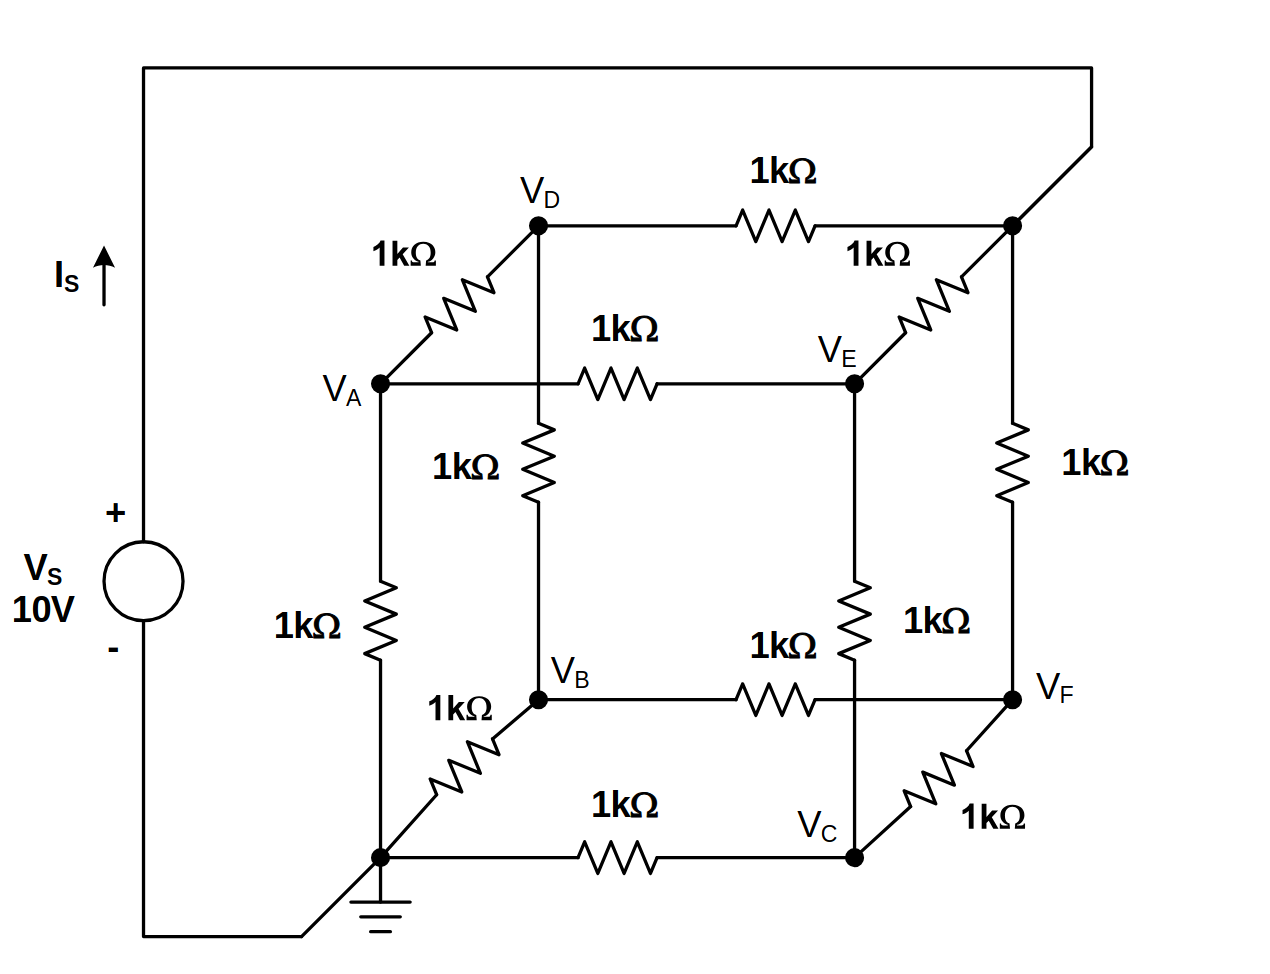
\includegraphics[width=\textwidth]{06_03}
	\caption{Cube.}
	\label{fig:circuit3}
\end{figure}
Notice that the current splits into three, then into 6, and finally back into 3
again before returning to ground. Using the knowledge that the current in any
node must always add up to $0A$ at any given time the total resistance can be
quickly calculated in terms of R as:
\[R_{eq} = R\frac{5}{6}\Omega\] which for a $1k\Omega$ value becomes:
\[
	R_{eq} = 833\Omega
\]
This results in a source current, $I_s$ of $12mA$.

Therefore, using the rules for combining resistances,
\[
	V_D = V_E = V_F = 10V - (I_s \cdot R) = 12mA \cdot 333.33\Omega = 10V - 4V = 6V\\
\]
\[
	V_A = V_B = V_C = 6V - (I_s \cdot R) = 12mA \cdot 166.67\Omega = 6V - 2V = 4V
\]
This completes the circuit analysis.
\section{Results and Discussion}
\subsection{Circuit One}
Referring back to the circuit in Figure \ref{fig:circuit1}, this simple circuit was realized
and analyzed in Scopy.

\subsubsection{Measured Response}
Due to the limitations of the ADALM2000, the following voltage was obtained at
$V_1$
\[
	V_1 = 1.749 V
\]
This is due to the voltages being scaled by a factor of $1/2$ down to adhere to
the five volt limit of the instrument. This is fine as there are no nonlinear
components that can't be scaled down.

When scaling this back up, however, the output is
\[
	V_1 \cdot 2 = 1.749 \cdot 2 = 3.498V
\]

\subsubsection{Assessment}
To assess the accuracy of the experimental result, we compute the percentage difference between the measured and calculated values using the following formula:

\[
	\text{Percentage Difference} = \left( \frac{|\text{Measured} - \text{Calculated}|}{\text{Calculated}} \right) \times 100
\]

\[
	= \left( \frac{|3.498\,\text{V} - 3.458\,\text{V}|}{3.458\,\text{V}} \right) \times 100 = \left( \frac{0.040\,\text{V}}{3.458\,\text{V}} \right) \times 100 \approx 1.16\%
\]

The measured value differs from the calculated value by approximately
\textbf{1.16\%}. This slight deviation can be attributed to the tolerance of the
resistors used which is $\pm 5\%$. This is in line with expectations.
\subsection{Circuit Two}
For this circuit, an additional power supply was used in order to more closely
match the conditions outlined in Figure \ref{fig:circuit2}.

\subsubsection{Measured Response}
This portion of the experimental work involved measuring the node voltages at
various values of $V_x$. Recall that $V_x$ has a negative polarity, which ends
up creating a larger magnitude in the negative direction for some of the
voltages felt at the nodes. Refer to Table \ref{table:measuredvolts} for the
data.

\begin{table}[H]
	\centering
	\begin{tabular}{|c|c|c|c|}
		\hline
		$V_x$ (V) & $V_1$ (V) & $V_2$ (V) & $V_3$ (V) \\
		\hline
		0         & 0.659     & 1.974     & 4.162     \\
		\hline
		0.5       & 0.332     & 1.784     & 4.109     \\
		\hline
		1.0       & -0.008    & 1.574     & 4.808     \\
		\hline
		1.5       & -0.354    & 1.355     & 3.908     \\
		\hline
		2.0       & -0.695    & 1.152     & 3.808     \\
		\hline
		2.5       & -1.046    & 0.933     & 3.691     \\
		\hline
		3.0       & -1.389    & 0.730     & 3.608     \\
		\hline
		3.5       & -1.738    & 0.506     & 3.474     \\
		\hline
		4.0       & -2.087    & 0.287     & 3.390     \\
		\hline
		4.5       & -2.589    & 0.068     & 3.307     \\
		\hline
		5.0       & -2.940    & -0.135    & 3.173     \\
		\hline
	\end{tabular}
	\caption{Measured Voltages}
	\label{table:measuredvolts}
\end{table}
The circuit was additionally crafted within the Spice simulation and node
values plotted
against the measured values as in Figure \ref{fig:measltspice}.
\begin{figure}[H]
	\centering
	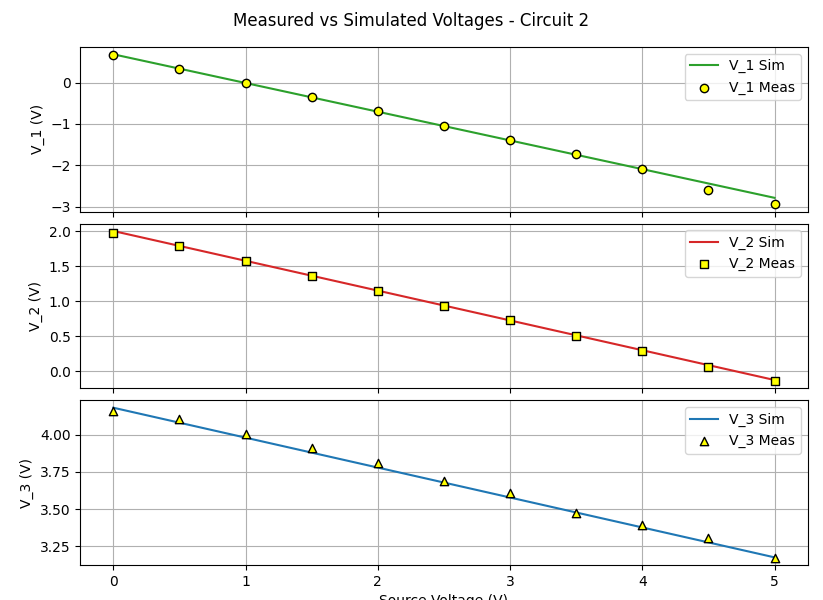
\includegraphics[height=8cm]{06_04}
	\caption{Simulated vs Measured Nodal Response}
	\label{fig:measltspice}
\end{figure}

The results not only match very closely, but they also trend in the exact same
linear way, with little deviation. This serves as a way to quickly
simulate the results, as well as allow for the verification of the realized
circuit.

\subsubsection{Assessment}
When comparing against the calculated values in the previous section,
\begin{align*}
	V_1          & = -2.788V    \\
	V_1_{PSpice} & = -2.788012V \\
	V_2          & = -0.124V    \\
	V_2_{PSpice} & = -0.123502V \\
	V_3          & = 3.174V     \\
	V_3_{PSpice} & = 3.174201V
\end{align*}
There are still small differences in values between them and the measured,
however the simulated results match these exactly as a result of the simulation
using the exact same techniques of nodal analysis, but in code rather than pen
and paper. This is a quite strong observation for further analysis.
\subsection{Circuit Three}

Building off of what was mentioned earlier about symmetry, the circuit can be
simplified by realizing that this is essentially a network of three series of
parallel resistor networks. The first has three resistors, the second has five,
and the third has three again. At each one of these nodes, Kirchhoff's Current
Law (KCL) determines an equal amount of current flowing into each respective
branch of the networks, due to all resistors being $1\,\text{k}\Omega$. Again,
an external source of 10V was utilized in order to account for the conditions of
the source figure.

Unfortunately, the school kit only allows for 10 $1\,\text{k}\Omega$ resistors.
To complete the cube,one parellel network of 3 $1k\Omega$ resistors was
substituded with a $330\,\Omega$ resistor. This slightly reduced the total equivalent resistance to approximately $830\,\Omega$ compared to the ideal theoretical value of $833\,\Omega$.

\subsubsection{Measured Response}

The following node voltages were measured experimentally:

\begin{align*}
	V_s             & = 10.000\ \text{V} \\
	V_A = V_B = V_C & = 3.758\ \text{V}  \\
	V_D = V_E = V_F & = 5.779\ \text{V}  \\
	I_s             & = 12.05\ \text{mA}
\end{align*}

Using Ohm’s Law, the experimental equivalent resistance between diagonal corners is:

\begin{align*}
	R_{\text{eq,exp}} & = \frac{V_s}{I_s} = \frac{10.000\ \text{V}}{12.05\ \text{mA}} = 830.29\ \Omega
\end{align*}

\subsubsection{SPICE Simulation Results}
In order to account more closely with the realized circuit, the final branch in
the simulator was also built to match the substituted resistor. With the
original values however, the theoretical results match perfectly to the
simulated ones, again due to the way in which SPICE simulation works.

The SPICE operating point simulation produced the following key values:
\begin{align*}
	V(n001) & = 10.000\ \text{V}  \\
	V(n002) & = 5.984\ \text{V}   \\
	V(n003) & = 3.976\ \text{V}   \\
	I(V_1)  & = -12.05\ \text{mA}
\end{align*}
These match the expected node behavior with top nodes around $5.98\ \text{V}$ and bottom nodes around $3.98\ \text{V}$, which is consistent with the symmetrical current splitting in the resistor cube network. The simulated current draw was:

\[
	I_s = 12.05\ \text{mA} \quad \Rightarrow \quad R_{\text{eq,sim}} = \frac{10.000\ \text{V}}{12.05\ \text{mA}} = 830.29\ \Omega
\]

\subsubsection{Assessment}
Recall, the theoretical equivalent resistance between two opposite corners of a symmetric resistor cube built from twelve $1\,\text{k}\Omega$ resistors is given by:
\[
	R_{\text{eq,theory}} = \frac{5}{6} \cdot R = \frac{5}{6}(1000\ \Omega) = 833.33\ \Omega
\]
All three values are in close agreement:

\begin{itemize}
	\item \textbf{Theoretical:} $833.33\ \Omega$
	\item \textbf{Simulated:} $830.29\ \Omega$
	\item \textbf{Experimental:} $830.29\ \Omega$
\end{itemize}

The less than $0.4\%$ deviation from the theoretical value is likely due to the resistor substitution and small measurement inaccuracies. Despite the missing resistors in the kit, both simulation and experiment successfully validated the cube’s behavior.

\section{Conclusion}
To conclude, the node voltage method is a powerful way to analyze and solve
circuits. Utilizing the extension of Kirchoff's Current Law, one can find the
node voltages at each essential node and solve for all of the missing values of
the components. Sometimes however, it is easier to just look at a circuit and do
some back of the napkin math as in circuit 3. Knowing symmetry alongside the
node voltage method an almost intuitive sense of the different circuit values
can be found merely by inspection. Nevertheless, as the tools to analyze
circuitry expand the node voltage method is a simple and surefire way that will
always work no matter what, so long as the passive sign convention is followed.
\end{document}
% vim: set ft=tex tw=80 ts=2 sts=2 sw=2 noet:
